\documentclass[1p]{elsarticle_modified}
%\bibliographystyle{elsarticle-num}

%\usepackage[colorlinks]{hyperref}
%\usepackage{abbrmath_seonhwa} %\Abb, \Ascr, \Acal ,\Abf, \Afrak
\usepackage{amsfonts}
\usepackage{amssymb}
\usepackage{amsmath}
\usepackage{amsthm}
\usepackage{scalefnt}
\usepackage{amsbsy}
\usepackage{kotex}
\usepackage{caption}
\usepackage{subfig}
\usepackage{color}
\usepackage{graphicx}
\usepackage{xcolor} %% white, black, red, green, blue, cyan, magenta, yellow
\usepackage{float}
\usepackage{setspace}
\usepackage{hyperref}

\usepackage{tikz}
\usetikzlibrary{arrows}

\usepackage{multirow}
\usepackage{array} % fixed length table
\usepackage{hhline}

%%%%%%%%%%%%%%%%%%%%%
\makeatletter
\renewcommand*\env@matrix[1][\arraystretch]{%
	\edef\arraystretch{#1}%
	\hskip -\arraycolsep
	\let\@ifnextchar\new@ifnextchar
	\array{*\c@MaxMatrixCols c}}
\makeatother %https://tex.stackexchange.com/questions/14071/how-can-i-increase-the-line-spacing-in-a-matrix
%%%%%%%%%%%%%%%

\usepackage[normalem]{ulem}

\newcommand{\msout}[1]{\ifmmode\text{\sout{\ensuremath{#1}}}\else\sout{#1}\fi}
%SOURCE: \msout is \stkout macro in https://tex.stackexchange.com/questions/20609/strikeout-in-math-mode

\newcommand{\cancel}[1]{
	\ifmmode
	{\color{red}\msout{#1}}
	\else
	{\color{red}\sout{#1}}
	\fi
}

\newcommand{\add}[1]{
	{\color{blue}\uwave{#1}}
}

\newcommand{\replace}[2]{
	\ifmmode
	{\color{red}\msout{#1}}{\color{blue}\uwave{#2}}
	\else
	{\color{red}\sout{#1}}{\color{blue}\uwave{#2}}
	\fi
}

\newcommand{\Sol}{\mathcal{S}} %segment
\newcommand{\D}{D} %diagram
\newcommand{\A}{\mathcal{A}} %arc


%%%%%%%%%%%%%%%%%%%%%%%%%%%%%5 test

\def\sl{\operatorname{\textup{SL}}(2,\Cbb)}
\def\psl{\operatorname{\textup{PSL}}(2,\Cbb)}
\def\quan{\mkern 1mu \triangleright \mkern 1mu}

\theoremstyle{definition}
\newtheorem{thm}{Theorem}[section]
\newtheorem{prop}[thm]{Proposition}
\newtheorem{lem}[thm]{Lemma}
\newtheorem{ques}[thm]{Question}
\newtheorem{cor}[thm]{Corollary}
\newtheorem{defn}[thm]{Definition}
\newtheorem{exam}[thm]{Example}
\newtheorem{rmk}[thm]{Remark}
\newtheorem{alg}[thm]{Algorithm}

\newcommand{\I}{\sqrt{-1}}
\begin{document}

%\begin{frontmatter}
%
%\title{Boundary parabolic representations of knots up to 8 crossings}
%
%%% Group authors per affiliation:
%\author{Yunhi Cho} 
%\address{Department of Mathematics, University of Seoul, Seoul, Korea}
%\ead{yhcho@uos.ac.kr}
%
%
%\author{Seonhwa Kim} %\fnref{s_kim}}
%\address{Center for Geometry and Physics, Institute for Basic Science, Pohang, 37673, Korea}
%\ead{ryeona17@ibs.re.kr}
%
%\author{Hyuk Kim}
%\address{Department of Mathematical Sciences, Seoul National University, Seoul 08826, Korea}
%\ead{hyukkim@snu.ac.kr}
%
%\author{Seokbeom Yoon}
%\address{Department of Mathematical Sciences, Seoul National University, Seoul, 08826,  Korea}
%\ead{sbyoon15@snu.ac.kr}
%
%\begin{abstract}
%We find all boundary parabolic representation of knots up to 8 crossings.
%
%\end{abstract}
%\begin{keyword}
%    \MSC[2010] 57M25 
%\end{keyword}
%
%\end{frontmatter}

%\linenumbers
%\tableofcontents
%
\newcommand\colored[1]{\textcolor{white}{\rule[-0.35ex]{0.8em}{1.4ex}}\kern-0.8em\color{red} #1}%
%\newcommand\colored[1]{\textcolor{white}{ #1}\kern-2.17ex	\textcolor{white}{ #1}\kern-1.81ex	\textcolor{white}{ #1}\kern-2.15ex\color{red}#1	}

{\Large $\underline{12a_{0582}~(K12a_{0582})}$}

\setlength{\tabcolsep}{10pt}
\renewcommand{\arraystretch}{1.6}
\vspace{1cm}\begin{tabular}{m{100pt}>{\centering\arraybackslash}m{274pt}}
\multirow{5}{120pt}{
	\centering
	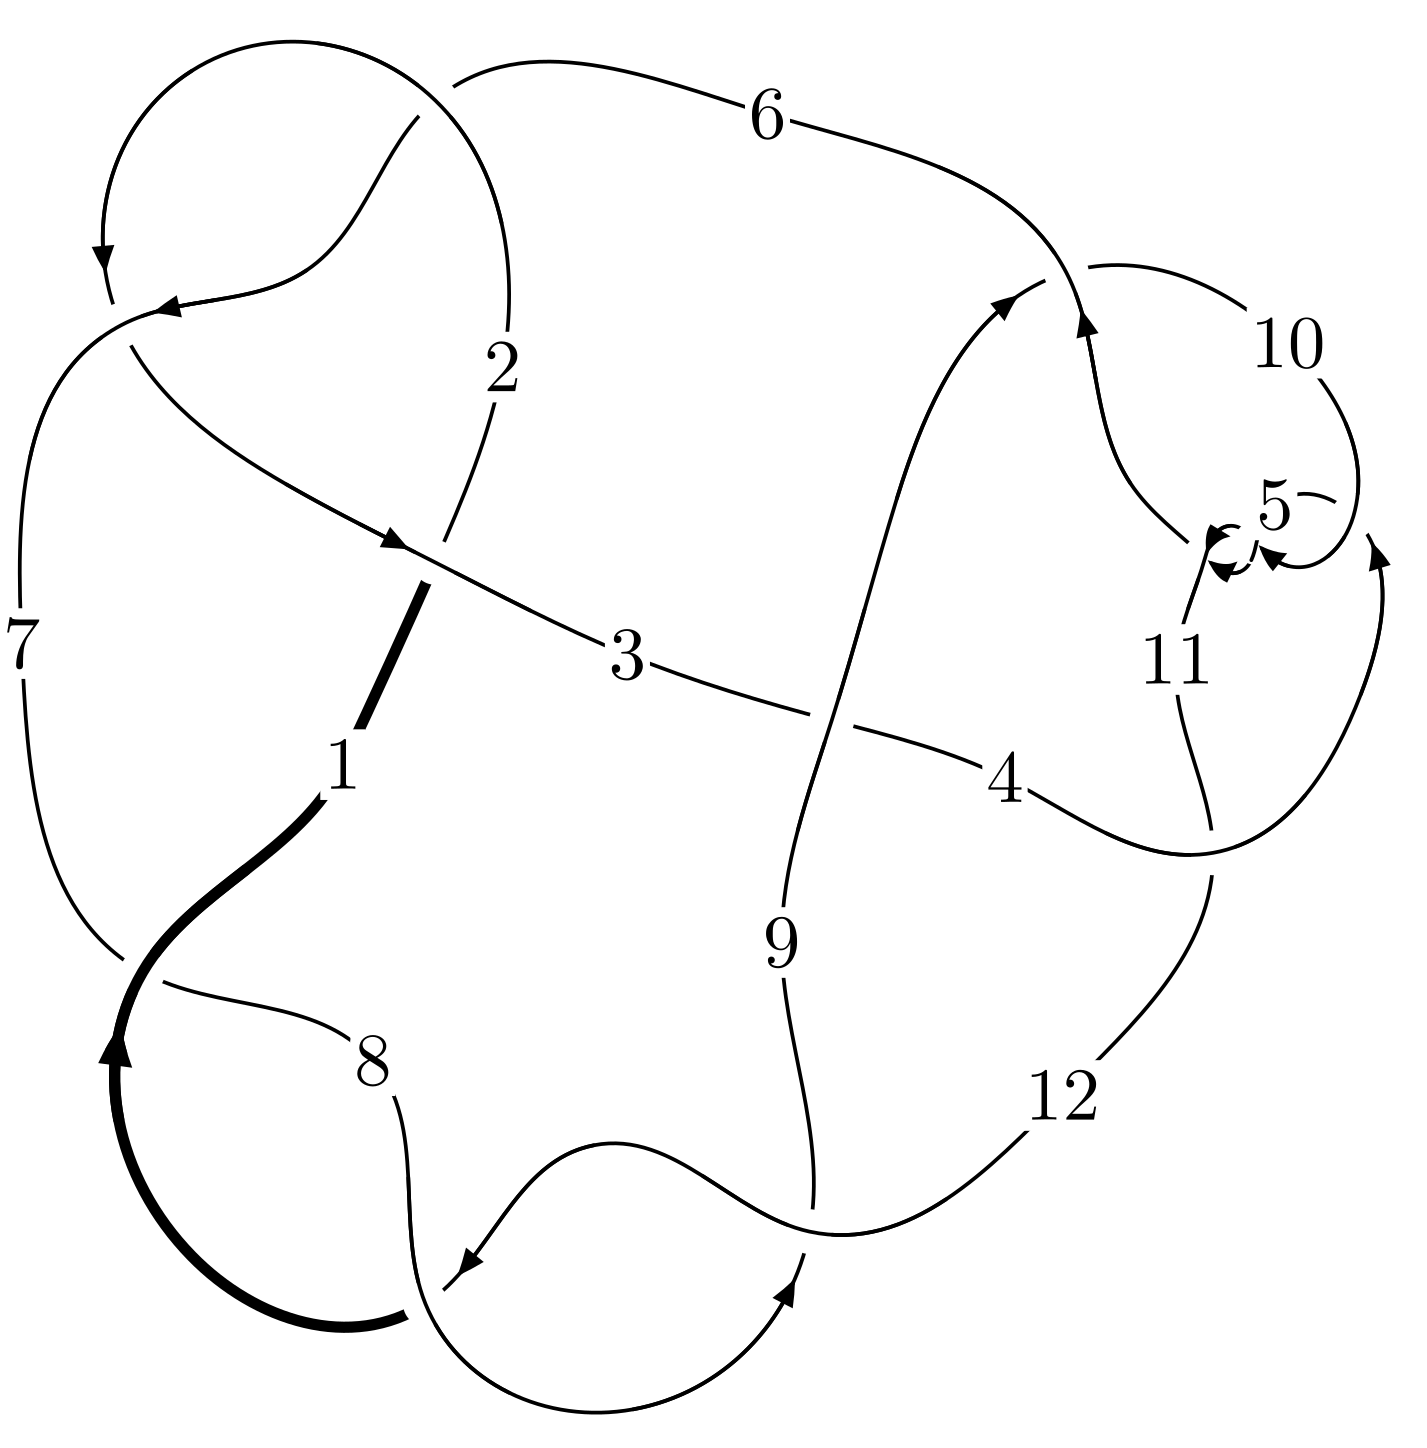
\includegraphics[width=112pt]{../../../GIT/diagram.site/Diagrams/png/1383_12a_0582.png}\\
\ \ \ A knot diagram\footnotemark}&
\allowdisplaybreaks
\textbf{Linearized knot diagam} \\
\cline{2-2}
 &
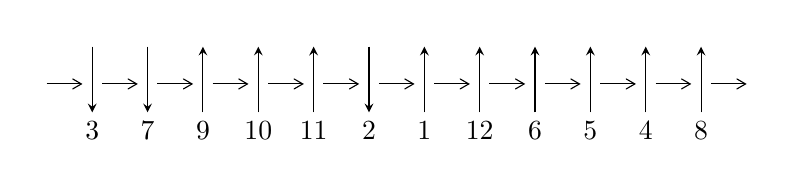
\begin{tikzpicture}[x=20pt, y=17pt]
	% nodes
	\node (C0) at (0, 0) {};
	\node (C1) at (1, 0) {};
	\node (C1U) at (1, +1) {};
	\node (C1D) at (1, -1) {3};

	\node (C2) at (2, 0) {};
	\node (C2U) at (2, +1) {};
	\node (C2D) at (2, -1) {7};

	\node (C3) at (3, 0) {};
	\node (C3U) at (3, +1) {};
	\node (C3D) at (3, -1) {9};

	\node (C4) at (4, 0) {};
	\node (C4U) at (4, +1) {};
	\node (C4D) at (4, -1) {10};

	\node (C5) at (5, 0) {};
	\node (C5U) at (5, +1) {};
	\node (C5D) at (5, -1) {11};

	\node (C6) at (6, 0) {};
	\node (C6U) at (6, +1) {};
	\node (C6D) at (6, -1) {2};

	\node (C7) at (7, 0) {};
	\node (C7U) at (7, +1) {};
	\node (C7D) at (7, -1) {1};

	\node (C8) at (8, 0) {};
	\node (C8U) at (8, +1) {};
	\node (C8D) at (8, -1) {12};

	\node (C9) at (9, 0) {};
	\node (C9U) at (9, +1) {};
	\node (C9D) at (9, -1) {6};

	\node (C10) at (10, 0) {};
	\node (C10U) at (10, +1) {};
	\node (C10D) at (10, -1) {5};

	\node (C11) at (11, 0) {};
	\node (C11U) at (11, +1) {};
	\node (C11D) at (11, -1) {4};

	\node (C12) at (12, 0) {};
	\node (C12U) at (12, +1) {};
	\node (C12D) at (12, -1) {8};
	\node (C13) at (13, 0) {};

	% arrows
	\draw[->,>={angle 60}]
	(C0) edge (C1) (C1) edge (C2) (C2) edge (C3) (C3) edge (C4) (C4) edge (C5) (C5) edge (C6) (C6) edge (C7) (C7) edge (C8) (C8) edge (C9) (C9) edge (C10) (C10) edge (C11) (C11) edge (C12) (C12) edge (C13) ;	\draw[->,>=stealth]
	(C1U) edge (C1D) (C2U) edge (C2D) (C3D) edge (C3U) (C4D) edge (C4U) (C5D) edge (C5U) (C6U) edge (C6D) (C7D) edge (C7U) (C8D) edge (C8U) (C9D) edge (C9U) (C10D) edge (C10U) (C11D) edge (C11U) (C12D) edge (C12U) ;
	\end{tikzpicture} \\
\hhline{~~} \\& 
\textbf{Solving Sequence} \\ \cline{2-2} 
 &
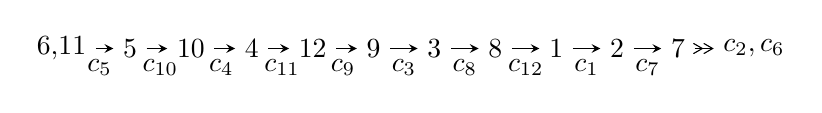
\begin{tikzpicture}[x=22pt, y=7pt]
	% node
	\node (A0) at (-1/8, 0) {6,11};
	\node (A1) at (1, 0) {5};
	\node (A2) at (2, 0) {10};
	\node (A3) at (3, 0) {4};
	\node (A4) at (4, 0) {12};
	\node (A5) at (5, 0) {9};
	\node (A6) at (6, 0) {3};
	\node (A7) at (7, 0) {8};
	\node (A8) at (8, 0) {1};
	\node (A9) at (9, 0) {2};
	\node (A10) at (10, 0) {7};
	\node (C1) at (1/2, -1) {$c_{5}$};
	\node (C2) at (3/2, -1) {$c_{10}$};
	\node (C3) at (5/2, -1) {$c_{4}$};
	\node (C4) at (7/2, -1) {$c_{11}$};
	\node (C5) at (9/2, -1) {$c_{9}$};
	\node (C6) at (11/2, -1) {$c_{3}$};
	\node (C7) at (13/2, -1) {$c_{8}$};
	\node (C8) at (15/2, -1) {$c_{12}$};
	\node (C9) at (17/2, -1) {$c_{1}$};
	\node (C10) at (19/2, -1) {$c_{7}$};
	\node (A11) at (45/4, 0) {$c_{2},c_{6}$};

	% edge
	\draw[->,>=stealth]	
	(A0) edge (A1) (A1) edge (A2) (A2) edge (A3) (A3) edge (A4) (A4) edge (A5) (A5) edge (A6) (A6) edge (A7) (A7) edge (A8) (A8) edge (A9) (A9) edge (A10) ;
	\draw[->>,>={angle 60}]	
	(A10) edge (A11);
\end{tikzpicture} \\ 

\end{tabular} \\

\footnotetext{
The image of knot diagram is generated by the software ``\textbf{Draw programme}" developed by Andrew Bartholomew(\url{http://www.layer8.co.uk/maths/draw/index.htm\#Running-draw}), where we modified some parts for our purpose(\url{https://github.com/CATsTAILs/LinksPainter}).
}\phantom \\ \newline 
\centering \textbf{Ideals for irreducible components\footnotemark of $X_{\text{par}}$} 
 
\begin{align*}
I^u_{1}&=\langle 
u^{65}- u^{64}+\cdots+u+1\rangle \\
\\
\end{align*}
\raggedright * 1 irreducible components of $\dim_{\mathbb{C}}=0$, with total 65 representations.\\
\footnotetext{All coefficients of polynomials are rational numbers. But the coefficients are sometimes approximated in decimal forms when there is not enough margin.}
\newpage
\renewcommand{\arraystretch}{1}
\centering \section*{I. $I^u_{1}= \langle u^{65}- u^{64}+\cdots+u+1 \rangle$}
\flushleft \textbf{(i) Arc colorings}\\
\begin{tabular}{m{7pt} m{180pt} m{7pt} m{180pt} }
\flushright $a_{6}=$&$\begin{pmatrix}1\\0\end{pmatrix}$ \\
\flushright $a_{11}=$&$\begin{pmatrix}0\\u\end{pmatrix}$ \\
\flushright $a_{5}=$&$\begin{pmatrix}1\\u^2\end{pmatrix}$ \\
\flushright $a_{10}=$&$\begin{pmatrix}- u\\- u^3+u\end{pmatrix}$ \\
\flushright $a_{4}=$&$\begin{pmatrix}- u^2+1\\- u^4+2 u^2\end{pmatrix}$ \\
\flushright $a_{12}=$&$\begin{pmatrix}u^5-2 u^3+u\\u^7-3 u^5+2 u^3+u\end{pmatrix}$ \\
\flushright $a_{9}=$&$\begin{pmatrix}u^3-2 u\\- u^3+u\end{pmatrix}$ \\
\flushright $a_{3}=$&$\begin{pmatrix}u^{10}-5 u^8+8 u^6-3 u^4-3 u^2+1\\- u^{10}+4 u^8-5 u^6+3 u^2\end{pmatrix}$ \\
\flushright $a_{8}=$&$\begin{pmatrix}u^{15}-6 u^{13}+14 u^{11}-14 u^9+2 u^7+6 u^5-2 u^3-2 u\\u^{17}-7 u^{15}+19 u^{13}-22 u^{11}+3 u^9+14 u^7-6 u^5-4 u^3+u\end{pmatrix}$ \\
\flushright $a_{1}=$&$\begin{pmatrix}u^{25}-10 u^{23}+\cdots+4 u^3+u\\u^{27}-11 u^{25}+\cdots- u^3+u\end{pmatrix}$ \\
\flushright $a_{2}=$&$\begin{pmatrix}- u^{47}+20 u^{45}+\cdots-8 u^5+14 u^3\\u^{47}-19 u^{45}+\cdots-4 u^3+u\end{pmatrix}$ \\
\flushright $a_{7}=$&$\begin{pmatrix}u^{35}-14 u^{33}+\cdots-5 u^3-2 u\\u^{37}-15 u^{35}+\cdots-7 u^3+u\end{pmatrix}$\\&\end{tabular}
\flushleft \textbf{(ii) Obstruction class $= -1$}\\~\\
\flushleft \textbf{(iii) Cusp Shapes $= -4 u^{63}+104 u^{61}+\cdots-8 u+10$}\\~\\
\newpage\renewcommand{\arraystretch}{1}
\flushleft \textbf{(iv) u-Polynomials at the component}\newline \\
\begin{tabular}{m{50pt}|m{274pt}}
Crossings & \hspace{64pt}u-Polynomials at each crossing \\
\hline $$\begin{aligned}c_{1}\end{aligned}$$&$\begin{aligned}
&u^{65}+37 u^{64}+\cdots+5 u+1
\end{aligned}$\\
\hline $$\begin{aligned}c_{2},c_{6}\end{aligned}$$&$\begin{aligned}
&u^{65}- u^{64}+\cdots+3 u-1
\end{aligned}$\\
\hline $$\begin{aligned}c_{3}\end{aligned}$$&$\begin{aligned}
&u^{65}- u^{64}+\cdots-975 u-1789
\end{aligned}$\\
\hline $$\begin{aligned}c_{4},c_{5},c_{10}\end{aligned}$$&$\begin{aligned}
&u^{65}+u^{64}+\cdots+u-1
\end{aligned}$\\
\hline $$\begin{aligned}c_{7},c_{8},c_{12}\end{aligned}$$&$\begin{aligned}
&u^{65}-3 u^{64}+\cdots+97 u-7
\end{aligned}$\\
\hline $$\begin{aligned}c_{9},c_{11}\end{aligned}$$&$\begin{aligned}
&u^{65}-3 u^{64}+\cdots-159 u+77
\end{aligned}$\\
\hline
\end{tabular}\\~\\
\newpage\renewcommand{\arraystretch}{1}
\flushleft \textbf{(v) Riley Polynomials at the component}\newline \\
\begin{tabular}{m{50pt}|m{274pt}}
Crossings & \hspace{64pt}Riley Polynomials at each crossing \\
\hline $$\begin{aligned}c_{1}\end{aligned}$$&$\begin{aligned}
&y^{65}-17 y^{64}+\cdots-23 y-1
\end{aligned}$\\
\hline $$\begin{aligned}c_{2},c_{6}\end{aligned}$$&$\begin{aligned}
&y^{65}-37 y^{64}+\cdots+5 y-1
\end{aligned}$\\
\hline $$\begin{aligned}c_{3}\end{aligned}$$&$\begin{aligned}
&y^{65}+23 y^{64}+\cdots-57349307 y-3200521
\end{aligned}$\\
\hline $$\begin{aligned}c_{4},c_{5},c_{10}\end{aligned}$$&$\begin{aligned}
&y^{65}-53 y^{64}+\cdots+5 y-1
\end{aligned}$\\
\hline $$\begin{aligned}c_{7},c_{8},c_{12}\end{aligned}$$&$\begin{aligned}
&y^{65}+71 y^{64}+\cdots+3781 y-49
\end{aligned}$\\
\hline $$\begin{aligned}c_{9},c_{11}\end{aligned}$$&$\begin{aligned}
&y^{65}+47 y^{64}+\cdots+71481 y-5929
\end{aligned}$\\
\hline
\end{tabular}\\~\\
\newpage\flushleft \textbf{(vi) Complex Volumes and Cusp Shapes}
$$\begin{array}{c|c|c}  
\text{Solutions to }I^u_{1}& \I (\text{vol} + \sqrt{-1}CS) & \text{Cusp shape}\\
 \hline 
\begin{aligned}
u &= -0.094573 + 0.834098 I\end{aligned}
 & -13.51750 - 0.44803 I & -2.98623 + 0.17507 I \\ \hline\begin{aligned}
u &= -0.094573 - 0.834098 I\end{aligned}
 & -13.51750 + 0.44803 I & -2.98623 - 0.17507 I \\ \hline\begin{aligned}
u &= -0.106309 + 0.831780 I\end{aligned}
 & -13.1248 - 9.9780 I & -2.29837 + 6.37976 I \\ \hline\begin{aligned}
u &= -0.106309 - 0.831780 I\end{aligned}
 & -13.1248 + 9.9780 I & -2.29837 - 6.37976 I \\ \hline\begin{aligned}
u &= \phantom{-}0.100233 + 0.828509 I\end{aligned}
 & -9.52777 + 5.06782 I & \phantom{-}0.64782 - 3.34296 I \\ \hline\begin{aligned}
u &= \phantom{-}0.100233 - 0.828509 I\end{aligned}
 & -9.52777 - 5.06782 I & \phantom{-}0.64782 + 3.34296 I \\ \hline\begin{aligned}
u &= \phantom{-}1.160000 + 0.299339 I\end{aligned}
 & -1.25708 - 2.56686 I & \phantom{-0.000000 } 0 \\ \hline\begin{aligned}
u &= \phantom{-}1.160000 - 0.299339 I\end{aligned}
 & -1.25708 + 2.56686 I & \phantom{-0.000000 } 0 \\ \hline\begin{aligned}
u &= \phantom{-}0.044240 + 0.791420 I\end{aligned}
 & -6.38103 + 0.21871 I & -4.02948 + 0.02486 I \\ \hline\begin{aligned}
u &= \phantom{-}0.044240 - 0.791420 I\end{aligned}
 & -6.38103 - 0.21871 I & -4.02948 - 0.02486 I \\ \hline\begin{aligned}
u &= -1.151480 + 0.383952 I\end{aligned}
 & -9.92789 + 5.59071 I & \phantom{-0.000000 } 0 \\ \hline\begin{aligned}
u &= -1.151480 - 0.383952 I\end{aligned}
 & -9.92789 - 5.59071 I & \phantom{-0.000000 } 0 \\ \hline\begin{aligned}
u &= \phantom{-}0.101141 + 0.776834 I\end{aligned}
 & -4.45615 + 6.50629 I & \phantom{-}0.43803 - 8.00885 I \\ \hline\begin{aligned}
u &= \phantom{-}0.101141 - 0.776834 I\end{aligned}
 & -4.45615 - 6.50629 I & \phantom{-}0.43803 + 8.00885 I \\ \hline\begin{aligned}
u &= \phantom{-}1.159270 + 0.378976 I\end{aligned}
 & -6.28819 - 0.70922 I & \phantom{-0.000000 } 0 \\ \hline\begin{aligned}
u &= \phantom{-}1.159270 - 0.378976 I\end{aligned}
 & -6.28819 + 0.70922 I & \phantom{-0.000000 } 0 \\ \hline\begin{aligned}
u &= -1.166850 + 0.385537 I\end{aligned}
 & -10.23340 - 3.94733 I & \phantom{-0.000000 } 0 \\ \hline\begin{aligned}
u &= -1.166850 - 0.385537 I\end{aligned}
 & -10.23340 + 3.94733 I & \phantom{-0.000000 } 0 \\ \hline\begin{aligned}
u &= -0.078114 + 0.754804 I\end{aligned}
 & -2.51311 - 2.38180 I & \phantom{-}3.80371 + 3.48935 I \\ \hline\begin{aligned}
u &= -0.078114 - 0.754804 I\end{aligned}
 & -2.51311 + 2.38180 I & \phantom{-}3.80371 - 3.48935 I \\ \hline\begin{aligned}
u &= -1.210410 + 0.285230 I\end{aligned}
 & \phantom{-}0.91435 - 1.38824 I & \phantom{-0.000000 } 0 \\ \hline\begin{aligned}
u &= -1.210410 - 0.285230 I\end{aligned}
 & \phantom{-}0.91435 + 1.38824 I & \phantom{-0.000000 } 0 \\ \hline\begin{aligned}
u &= -1.25678\phantom{ +0.000000I}\end{aligned}
 & \phantom{-}2.32752\phantom{ +0.000000I} & \phantom{-0.000000 } 0 \\ \hline\begin{aligned}
u &= \phantom{-}1.225780 + 0.337681 I\end{aligned}
 & -2.74836 + 3.85748 I & \phantom{-0.000000 } 0 \\ \hline\begin{aligned}
u &= \phantom{-}1.225780 - 0.337681 I\end{aligned}
 & -2.74836 - 3.85748 I & \phantom{-0.000000 } 0 \\ \hline\begin{aligned}
u &= -0.048386 + 0.684959 I\end{aligned}
 & -1.42383 - 1.84364 I & \phantom{-}4.80084 + 4.67821 I \\ \hline\begin{aligned}
u &= -0.048386 - 0.684959 I\end{aligned}
 & -1.42383 + 1.84364 I & \phantom{-}4.80084 - 4.67821 I \\ \hline\begin{aligned}
u &= -1.287820 + 0.269388 I\end{aligned}
 & \phantom{-}2.46404 - 1.51677 I & \phantom{-0.000000 } 0 \\ \hline\begin{aligned}
u &= -1.287820 - 0.269388 I\end{aligned}
 & \phantom{-}2.46404 + 1.51677 I & \phantom{-0.000000 } 0 \\ \hline\begin{aligned}
u &= \phantom{-}1.307270 + 0.296498 I\end{aligned}
 & \phantom{-}2.83926 + 5.43289 I & \phantom{-0.000000 } 0\\
 \hline 
 \end{array}$$\newpage$$\begin{array}{c|c|c}  
\text{Solutions to }I^u_{1}& \I (\text{vol} + \sqrt{-1}CS) & \text{Cusp shape}\\
 \hline 
\begin{aligned}
u &= \phantom{-}1.307270 - 0.296498 I\end{aligned}
 & \phantom{-}2.83926 - 5.43289 I & \phantom{-0.000000 } 0 \\ \hline\begin{aligned}
u &= -1.296820 + 0.344926 I\end{aligned}
 & -2.19604 - 4.31467 I & \phantom{-0.000000 } 0 \\ \hline\begin{aligned}
u &= -1.296820 - 0.344926 I\end{aligned}
 & -2.19604 + 4.31467 I & \phantom{-0.000000 } 0 \\ \hline\begin{aligned}
u &= \phantom{-}1.348140 + 0.018843 I\end{aligned}
 & \phantom{-}6.21518 + 0.45322 I & \phantom{-0.000000 } 0 \\ \hline\begin{aligned}
u &= \phantom{-}1.348140 - 0.018843 I\end{aligned}
 & \phantom{-}6.21518 - 0.45322 I & \phantom{-0.000000 } 0 \\ \hline\begin{aligned}
u &= -0.460545 + 0.448848 I\end{aligned}
 & -7.99941 - 6.33251 I & \phantom{-}0.97978 + 6.99711 I \\ \hline\begin{aligned}
u &= -0.460545 - 0.448848 I\end{aligned}
 & -7.99941 + 6.33251 I & \phantom{-}0.97978 - 6.99711 I \\ \hline\begin{aligned}
u &= \phantom{-}1.318160 + 0.325546 I\end{aligned}
 & \phantom{-}1.86620 + 6.29334 I & \phantom{-0.000000 } 0 \\ \hline\begin{aligned}
u &= \phantom{-}1.318160 - 0.325546 I\end{aligned}
 & \phantom{-}1.86620 - 6.29334 I & \phantom{-0.000000 } 0 \\ \hline\begin{aligned}
u &= -1.357310 + 0.046814 I\end{aligned}
 & \phantom{-}4.98134 - 4.45057 I & \phantom{-0.000000 } 0 \\ \hline\begin{aligned}
u &= -1.357310 - 0.046814 I\end{aligned}
 & \phantom{-}4.98134 + 4.45057 I & \phantom{-0.000000 } 0 \\ \hline\begin{aligned}
u &= -1.360890 + 0.109523 I\end{aligned}
 & \phantom{-}1.21860 - 3.40283 I & \phantom{-0.000000 } 0 \\ \hline\begin{aligned}
u &= -1.360890 - 0.109523 I\end{aligned}
 & \phantom{-}1.21860 + 3.40283 I & \phantom{-0.000000 } 0 \\ \hline\begin{aligned}
u &= \phantom{-}1.359500 + 0.126402 I\end{aligned}
 & -2.55503 - 1.02133 I & \phantom{-0.000000 } 0 \\ \hline\begin{aligned}
u &= \phantom{-}1.359500 - 0.126402 I\end{aligned}
 & -2.55503 + 1.02133 I & \phantom{-0.000000 } 0 \\ \hline\begin{aligned}
u &= -0.424540 + 0.468915 I\end{aligned}
 & -8.11205 + 2.96450 I & \phantom{-}0.512038 + 0.590116 I \\ \hline\begin{aligned}
u &= -0.424540 - 0.468915 I\end{aligned}
 & -8.11205 - 2.96450 I & \phantom{-}0.512038 - 0.590116 I \\ \hline\begin{aligned}
u &= -1.329800 + 0.335920 I\end{aligned}
 & \phantom{-}0.03580 - 10.52840 I & \phantom{-0.000000 } 0 \\ \hline\begin{aligned}
u &= -1.329800 - 0.335920 I\end{aligned}
 & \phantom{-}0.03580 + 10.52840 I & \phantom{-0.000000 } 0 \\ \hline\begin{aligned}
u &= \phantom{-}1.373990 + 0.109382 I\end{aligned}
 & -2.26088 + 8.10639 I & \phantom{-0.000000 } 0 \\ \hline\begin{aligned}
u &= \phantom{-}1.373990 - 0.109382 I\end{aligned}
 & -2.26088 - 8.10639 I & \phantom{-0.000000 } 0 \\ \hline\begin{aligned}
u &= \phantom{-}0.434819 + 0.442821 I\end{aligned}
 & -4.36631 + 1.63515 I & \phantom{-}4.04889 - 3.95460 I \\ \hline\begin{aligned}
u &= \phantom{-}0.434819 - 0.442821 I\end{aligned}
 & -4.36631 - 1.63515 I & \phantom{-}4.04889 + 3.95460 I \\ \hline\begin{aligned}
u &= \phantom{-}1.331870 + 0.368474 I\end{aligned}
 & -9.04383 + 4.77398 I & \phantom{-0.000000 } 0 \\ \hline\begin{aligned}
u &= \phantom{-}1.331870 - 0.368474 I\end{aligned}
 & -9.04383 - 4.77398 I & \phantom{-0.000000 } 0 \\ \hline\begin{aligned}
u &= -1.334750 + 0.364272 I\end{aligned}
 & -5.02433 - 9.36081 I & \phantom{-0.000000 } 0 \\ \hline\begin{aligned}
u &= -1.334750 - 0.364272 I\end{aligned}
 & -5.02433 + 9.36081 I & \phantom{-0.000000 } 0 \\ \hline\begin{aligned}
u &= \phantom{-}1.338820 + 0.365504 I\end{aligned}
 & -8.5870 + 14.2869 I & \phantom{-0.000000 } 0 \\ \hline\begin{aligned}
u &= \phantom{-}1.338820 - 0.365504 I\end{aligned}
 & -8.5870 - 14.2869 I & \phantom{-0.000000 } 0 \\ \hline\begin{aligned}
u &= \phantom{-}0.466465 + 0.249612 I\end{aligned}
 & -0.58098 + 3.59821 I & \phantom{-}5.77066 - 8.87995 I\\
 \hline 
 \end{array}$$\newpage$$\begin{array}{c|c|c}  
\text{Solutions to }I^u_{1}& \I (\text{vol} + \sqrt{-1}CS) & \text{Cusp shape}\\
 \hline 
\begin{aligned}
u &= \phantom{-}0.466465 - 0.249612 I\end{aligned}
 & -0.58098 - 3.59821 I & \phantom{-}5.77066 + 8.87995 I \\ \hline\begin{aligned}
u &= \phantom{-}0.188336 + 0.389034 I\end{aligned}
 & -1.44853 - 1.18673 I & \phantom{-}0.463992 + 0.219440 I \\ \hline\begin{aligned}
u &= \phantom{-}0.188336 - 0.389034 I\end{aligned}
 & -1.44853 + 1.18673 I & \phantom{-}0.463992 - 0.219440 I \\ \hline\begin{aligned}
u &= -0.421061 + 0.080852 I\end{aligned}
 & \phantom{-}0.842001 - 0.137199 I & \phantom{-}12.42572 + 1.52219 I \\ \hline\begin{aligned}
u &= -0.421061 - 0.080852 I\end{aligned}
 & \phantom{-}0.842001 + 0.137199 I & \phantom{-}12.42572 - 1.52219 I\\
 \hline 
 \end{array}$$\newpage
\newpage\renewcommand{\arraystretch}{1}
\centering \section*{ II. u-Polynomials}
\begin{tabular}{m{50pt}|m{274pt}}
Crossings & \hspace{64pt}u-Polynomials at each crossing \\
\hline $$\begin{aligned}c_{1}\end{aligned}$$&$\begin{aligned}
&u^{65}+37 u^{64}+\cdots+5 u+1
\end{aligned}$\\
\hline $$\begin{aligned}c_{2},c_{6}\end{aligned}$$&$\begin{aligned}
&u^{65}- u^{64}+\cdots+3 u-1
\end{aligned}$\\
\hline $$\begin{aligned}c_{3}\end{aligned}$$&$\begin{aligned}
&u^{65}- u^{64}+\cdots-975 u-1789
\end{aligned}$\\
\hline $$\begin{aligned}c_{4},c_{5},c_{10}\end{aligned}$$&$\begin{aligned}
&u^{65}+u^{64}+\cdots+u-1
\end{aligned}$\\
\hline $$\begin{aligned}c_{7},c_{8},c_{12}\end{aligned}$$&$\begin{aligned}
&u^{65}-3 u^{64}+\cdots+97 u-7
\end{aligned}$\\
\hline $$\begin{aligned}c_{9},c_{11}\end{aligned}$$&$\begin{aligned}
&u^{65}-3 u^{64}+\cdots-159 u+77
\end{aligned}$\\
\hline
\end{tabular}\newpage\renewcommand{\arraystretch}{1}
\centering \section*{ III. Riley Polynomials}
\begin{tabular}{m{50pt}|m{274pt}}
Crossings & \hspace{64pt}Riley Polynomials at each crossing \\
\hline $$\begin{aligned}c_{1}\end{aligned}$$&$\begin{aligned}
&y^{65}-17 y^{64}+\cdots-23 y-1
\end{aligned}$\\
\hline $$\begin{aligned}c_{2},c_{6}\end{aligned}$$&$\begin{aligned}
&y^{65}-37 y^{64}+\cdots+5 y-1
\end{aligned}$\\
\hline $$\begin{aligned}c_{3}\end{aligned}$$&$\begin{aligned}
&y^{65}+23 y^{64}+\cdots-57349307 y-3200521
\end{aligned}$\\
\hline $$\begin{aligned}c_{4},c_{5},c_{10}\end{aligned}$$&$\begin{aligned}
&y^{65}-53 y^{64}+\cdots+5 y-1
\end{aligned}$\\
\hline $$\begin{aligned}c_{7},c_{8},c_{12}\end{aligned}$$&$\begin{aligned}
&y^{65}+71 y^{64}+\cdots+3781 y-49
\end{aligned}$\\
\hline $$\begin{aligned}c_{9},c_{11}\end{aligned}$$&$\begin{aligned}
&y^{65}+47 y^{64}+\cdots+71481 y-5929
\end{aligned}$\\
\hline
\end{tabular}
\vskip 2pc
\end{document}